\chapter{Resultater og analyse fra Case 3: Misbruk av NTNU sin infrastruktur til utvinning av kryptovaluta}
I dette kapittelet fremlegger vi våre resultater i alle fasene i case 3.
%%%%%%%%%%%%%%%%%%%%%%%%%%%%%%%%%%%%%%%%%%%%%%%%%%%%%%%%%%%%%%%%%%%%%
\section{Problemforståelse}
\subsection{Ytelsesmatrise}
Variablene som ble vurdert til å kunne hjelpe til å redusere utvinning av kryptovaluta hos NTNU er som følger:
\begin{description}
    \item[Adgangskontroll på HPC klynger:] Klynger av tilkoblet maskinvare som sammen utgir svært høy ytelse. Er også kjent som superdatamaskiner. Disse er godt beskyttet med streng adgangskontroll og logging av alt som blir gjort.
    \item[Adgangskontroll på kritiske servere:] Adgangskontroll til servere som har en funksjonskritisk og/eller virksomhetskritisk rolle i driften av NTNU, som for eksempel DNS og DHCP servere. 
    \item[Adgangskontroll på andre servere:] Adgangskontroll til alle servere som ikke har en kritisk rolle i NTNU, men som fortsatt kan bli misbrukt. Inkluderer servere som står åpent ut mot nettet. 
    \item[Beskyttelse mot ufrivillig utvinning på datamaskiner:] Beskyttelse mot at personer får tilgang til din datamaskin gjennom nettleseren og bruker den til å utvinne kryptovaluta. 
    \item[Policy på hva som er akseptabelt som BYOD:] Definerer hva som er lov å ta med av BYOD.
    \item[IT-reglement på kryptoutvinning:] IT-reglementet spesifiserer per i dag bare at det å misbruke universitetets ressurser til kommersiell virksomhet ikke er greit. Det kan være vanskelig for folk å skjønne at strøm er en slik ressurs og at utvinning av kryptovaluta kan regnes som kommersiell virksomhet. Slik som IT-reglementet er idag er det heller ikke noen gode sanksjonsmuligheter mot folk som utvinner kryptovaluta.
\end{description}

Under ser vi hvor de ulike ressursene, eller aktiva, er plassert i henhold til de tidligere nevnte områdene.
\begin{figure}[H]
    \centering
    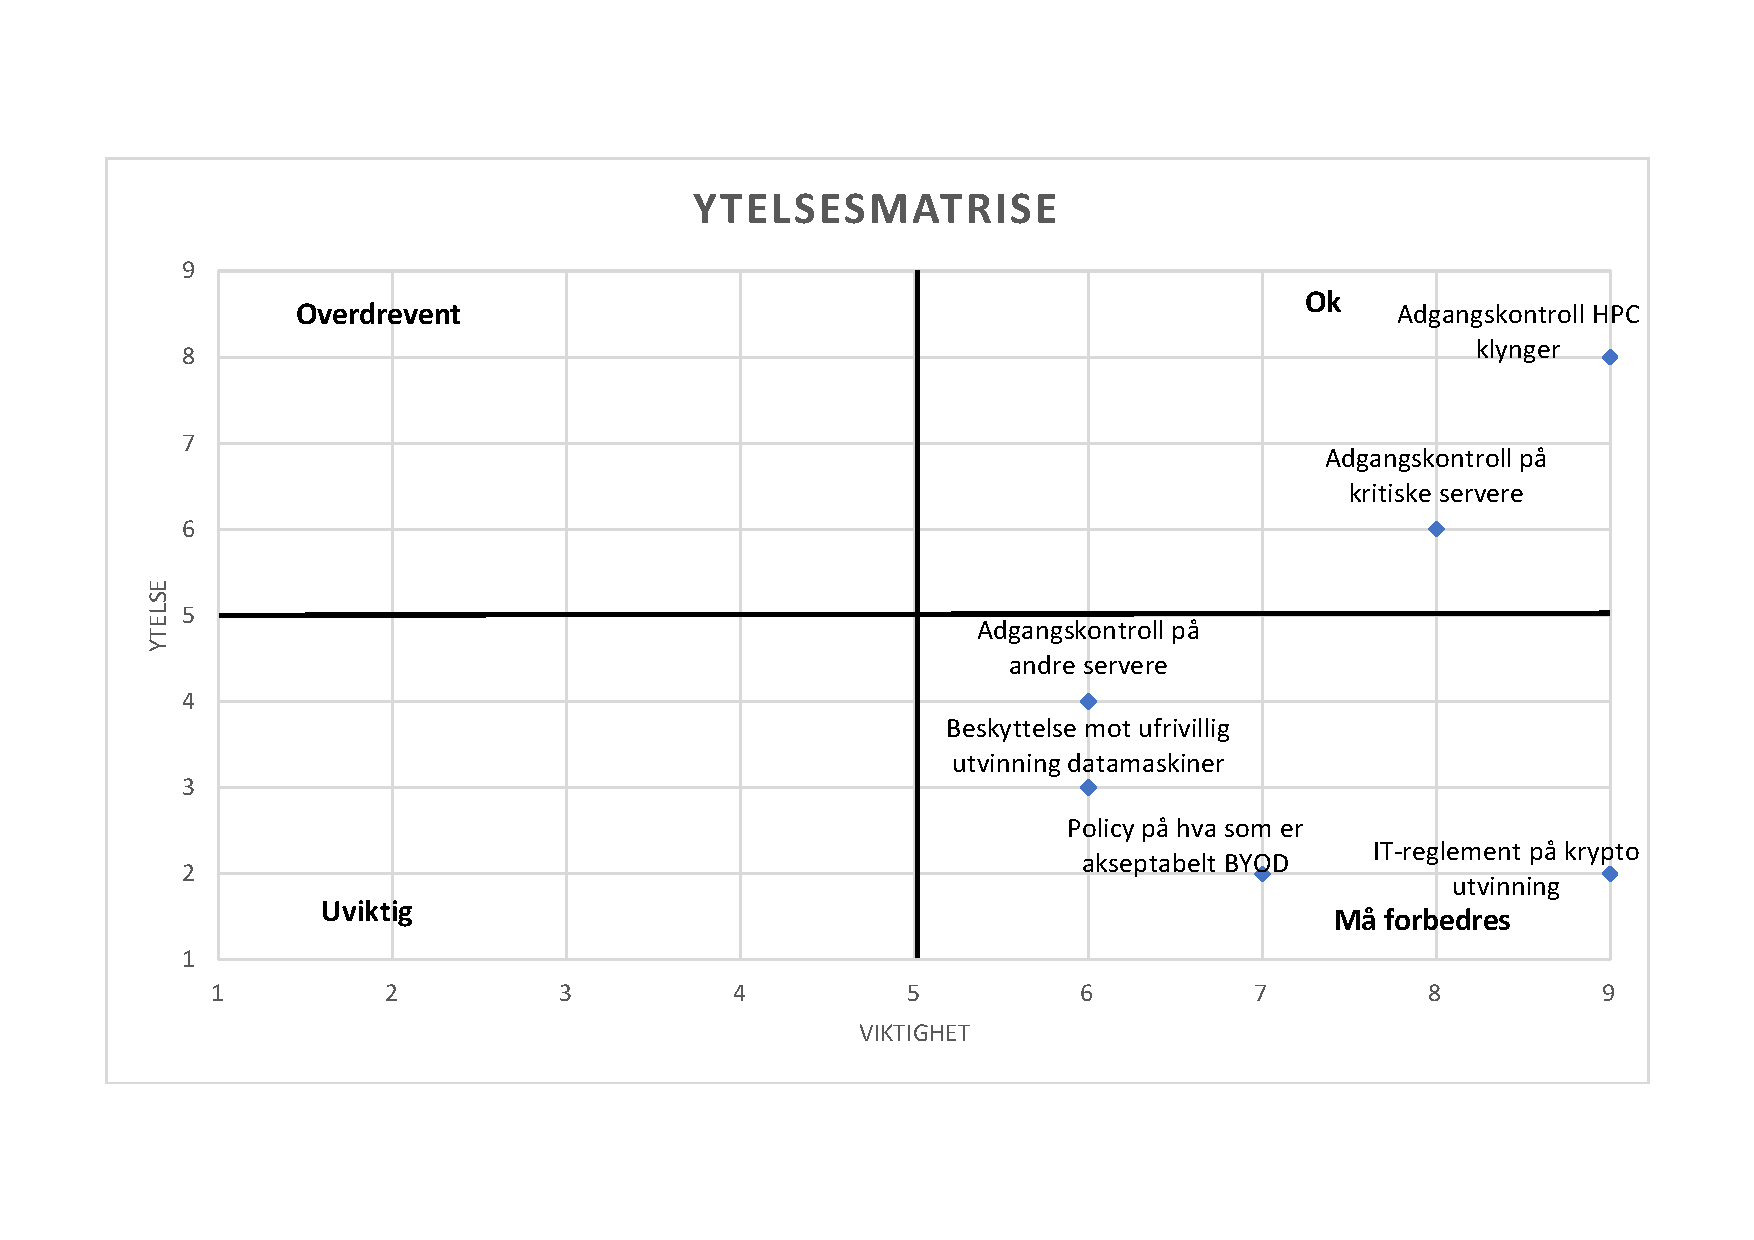
\includegraphics[scale=0.5]{case_3/bilder/ytelsesmatrise.pdf}
    \caption[Ytelsesmatrise]{Resultater fra ytelsesmatrisen}
    \label{fig:ytelsesmatrise}
\end{figure}

Det er mest kritisk å vurdere de variablene som havner under ``må forbedres''. Selv om noen havner under ``ok'', bør de fortsatt vurderes, men de vil ha lavere prioritet enn de nevnt over. Variabler som er uviktig eller overdrevent trenger man ikke vurdere nøye. Matrisen viser følgende prioriteringsgrunnlag til utbedring:

\begin{enumerate}
    \item IT-reglement på kryptoutvinning
    \item Policy på hva som er akseptabelt som BYOD
    \item Beskyttelse mot ufrivillig utvinning på datamaskiner
    \item Adgangskontroll på andre servere
    \item Adgangskontroll på kritiske servere
    \item Adgangskontroll på HPC klynger
\end{enumerate}

%%%%%%%%%%%%%%%%%%%%%%%%%%%%%%%%%%%%%%%%%%%%%%%%%%%%%%%%%%%%%%%%%%%%%
\section{Idémyldring}
\subsection{Idémyldring}
Etter at idémyldringsøkten var ferdig ble det gjort en vurdering av hvilke momenter som hørte sammen eller hadde likhetstrekk.  Disse ble gruppert sammen, se figur \ref{fig:idemyldring-hvordan} og \ref{fig:idemyldring-hvorfor} under.

\begin{figure}[H]
    \centering
    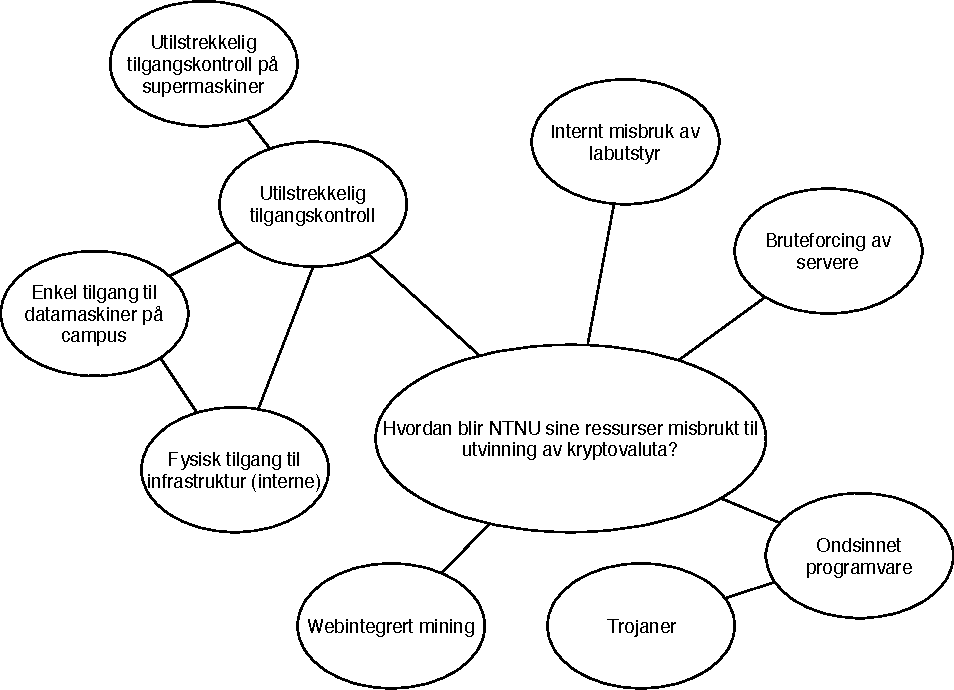
\includegraphics[scale=0.6]{case_3/bilder/idemyldring-hvordan.pdf}
    \caption[Idémyldring hvordan]{Resultater og gruppering av Hvordan}
     \label{fig:idemyldring-hvordan}
\end{figure}

\begin{figure}[H]
    \centering
    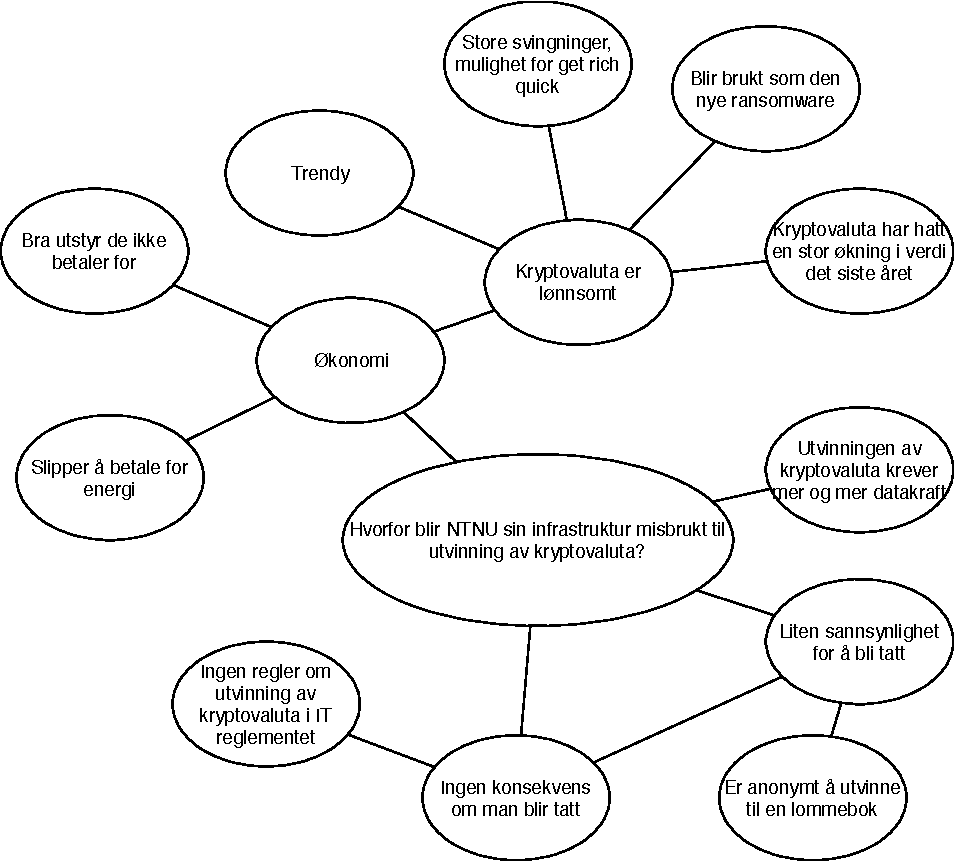
\includegraphics[scale=0.6]{case_3/bilder/idemyldring-hvorfor.pdf}
    \caption[Idémyldring hvorfor]{Resultater og gruppering av Hvorfor}
    \label{fig:idemyldring-hvorfor}
\end{figure}

Resultatene er gruppert inn i 4 hovedkategorier:
\begin{description}
    \item [Ondsinnet programmvare] Er i stor grad trojanere i form av javascript.
    \item [Utilstrekkelig tilgangskontroll] Tilganskontroll på diverese datamaskiner rundt på campus, som kan utnyttes.
    \item [Økonomi] Er i stor grad motivasjonen til aktørene, der det er stor økonomisk vinning med kryptovaluta.
    \item[Ingen konsekvens om man blir tatt] Det står lite i IT-reglementet om at kryptoutvinning ikke er lov.
\end{description}

\subsection{NGT}
Etter at hvert gruppemedlem hadde gitt ut sine 15 poeng satt vi igjen med 4 idéer som stakk seg ut med hvor mange poeng de fikk. Disse vises i fet skrift i tabell \ref{tab:NGT}. 

\begin{table} [H]
    \begin{tabular}{ | m{2em} | m{30em} | m{3em} | }
        \hline
            \cellcolor{yellow}  & \cellcolor{yellow} \textbf{Årsak} & \cellcolor{yellow} Poeng \\
        \hline
           A& Bra utstyr de ikke betaler for & 5 \\
        \hline
          B & Bruteforce av servere & 0 \\
        \hline
          C & Enkel tilgang til datamaskiner på campus & 0 \\
        \hline
         \textbf{D} & \textbf{Ingen regler om utvinning av kryptovaluta i IT-reglementet} & 11 \\
        \hline
          \textbf{E} & \textbf{Internt misbruk av labutstyr} & 8  \\
        \hline
          F & Kryptovaluta har hatt en stor økning i verdi det siste året & 0 \\
        \hline
         G & Liten sannsynlighet for å bli tatt & 2 \\
        \hline
         \textbf{H} & \textbf{Ondsinnet programvare som utvinner} &  16 \\
        \hline
         I & Slipper å betale for energi & 0 \\
        \hline
         J & Store svingninger, mulighet for “get rich quick" & 0 \\
        \hline
         K & Utilstrekkelig tilgangskontroll på supermaskiner & 0 \\
        \hline
         L & Utvinningen av kryptovaluta krever mer og mer datakraft & 4 \\
        \hline
         \textbf{M} & \textbf{Kryptoutvinner integrert i nettleser} & 14 \\
        \hline
    \end{tabular}
    \caption{Oversikt over prioritering av idéer ved hjelp av NGT}
    \label{tab:NGT}
\end{table}

Disse fire årsakene er de vi kommer til å fokusere på i dette caset. De fire fokuspunktene kan deles etter de to problemstillingene ``hvordan og hvorfor''.

De to årsakene knyttet til ``hvorfor'' går ut på at det ikke er ulovlig med kryptoutvinning i henhold til gjeldende regelverk \cite{ITReg}. De faller derfor i en gråsone der en ikke får noen represalier for å holde på med kryptoutvinning, annet enn å bli kastet av nettet. Konsekvensene får man hvis en utnytter NTNU sine ressurser til egen vinning.

De neste årsakene går ut på hvilke aktører som bruker universitetet sine ressurser til utvinning av kryptovaluta, og hvordan de bruker ressursene. Internt misbruk av labutstyr går ut på at studenter eller ansatte har tilgang til diverse labber og PCer som kan brukes til utvinning av kryptovaluta. Både ondsinnet programvare som utvinner kryptovaluta og kryptoutvinnere integrert i nettleser brukes av eksterne trusselaktører. Pengene som tjenes her går til kriminelle. Utvinning av kryptovaluta har blitt mer utbredt som et alternativ til løsepengevirus, der løsepengevirus har blitt mindre lønnsomt den siste tiden \cite{RW}.

%%%%%%%%%%%%%%%%%%%%%%%%%%%%%%%%%%%%%%%%%%%%%%%%%%%%%%%%%%%%%%%%%%%%%
\section{Datainnsamling}
\subsection{Spørreundersøkelse}
Før intervjuet fikk vi et utdrag av alarmer som SOCen får av de kjente signaturene som omhandler kryotoutvinning. Disse alarmene stammer fra kryptoutvinnere som folk har fått lagt inn på PCene sine, kryptoutvinnere i nettleser som er lagt inn på diverse nettsteder eller trojanere. 

Vi hadde noen hypoteser når vi utformet intervjuspørsmålene, disse var:
\begin{itemize}
    \item Det er tekniske løsninger som kan brukes til å fikse store deler av problemet.
    \item Det er begrenset handlingsrom for hva som kan bli gjort mot interne som utvinner.
    \item Lite bevissthet rundt regelverket til NTNU angående bruk av universitetets ressurser.
    \item Utviklingen av utvinning følger kryptovalutaen sin verdi.
    \item Dataer blir kompromittert gjennom de vanlige formene, phishing og wateringholes.
\end{itemize}

\begin{table}[H]
    \centering
    \begin{tabular}{|m{30em}|} 
        \hline
        \cellcolor{yellow} Spørsmål  \\
        \hline
        Hva er de typiske angrepsvektorene?  \\
        \hline
        Tar det lang tid å oppdage trojanere i nettverket? \\ 
        \hline
        Hva gjør Seksjon for Digital Sikkerhet når de oppdager trojanere? \\
        \hline
        Hvordan fant dere ut om HPC clusterne blir misbrukt? \\
        \hline
        Hvordan fant dere ut at det var internt misbruk?\\
        \hline
        Har dere andre tiltak enn å stenge internett til de som miner? \\
        \hline
        hva er grunnen til at dere ikke har implementert noe slike tiltak? \\
        \hline
        Hva tror du er oppfatningen blant dine kolleger er angående utvinning. Vet folk det er ulovlig eller har de ikke tenkt så mye over det og utvinner fordi det er en trend? \\
        \hline
        Hva er måten dere for du snakket tidligere om at dere så mange av de lommebøkene som ble brukt var fra mørke siden av nettet?  \\
        \hline
        Hvordan ser dere at de går til disse lommebøkene? \\
        \hline
        Hvordan skal dere implementere kryptoutvinning i neste IT-reglement? \\
        \hline
        Tenker folk over at det ikke er lov til å utvinne kryptovaluta i henhold til IT-reglementet? \\
        \hline
        Har dere noen tiltak på utvinning på nettsider? \\
        \hline
        Er det like stor økning nå som det var før jul? \\
        \hline
        Økningen er det gjort av de profesjonelle aktørene eller er det folk som setter frivillig opp utvinnere? \\
        \hline
        Dere hadde ikke sett noe tilfeller av bruteforcede PCer og servere som ble installert kryptominere på, etter at de ble bruteforcet?  \\
        \hline
        Er det noen regler på hva ansatte får lov til å legge på serverne? \\
        \hline
        Har dere noen tilfeller av PCer på datalabber der studenter har installert kryptoutvinning? \\
        \hline
    \end{tabular}
    \caption{Spørsmål til intervju case 3}
    \label{tab:spm-intervju}
\end{table}
Under intervjuet ble det tatt lydopptak, slik at vi lett kunne gå tilbake til svarene for å få det mest mulig nøyaktig til neste fase. Når intervjuet var ferdig ble det transkribert. Transkripsjonen finnes i vedlegg \ref{transkripsjon}.
%%%%%%%%%%%%%%%%%%%%%%%%%%%%%%%%%%%%%%%%%%%%%%%%%%%%%%%%%%%%%%%%%%%%%
\section{Dataanalyse}
\subsection{Affinitetsdiagram}
Affinitetsdiagram brukes til å analysere data som det ikke er mulig å nummerere, eksempelvis meninger eller idéer. Affinitetsdiagram grupperer data og finner de underliggende korrelasjoner og likhetstrekk i gruppen.

Analysen ble gjennomført med å ta transkripsjon av intervjuet og stykke den opp i fem hovedgrupper.     

\begin{figure}[H]
    \centering
    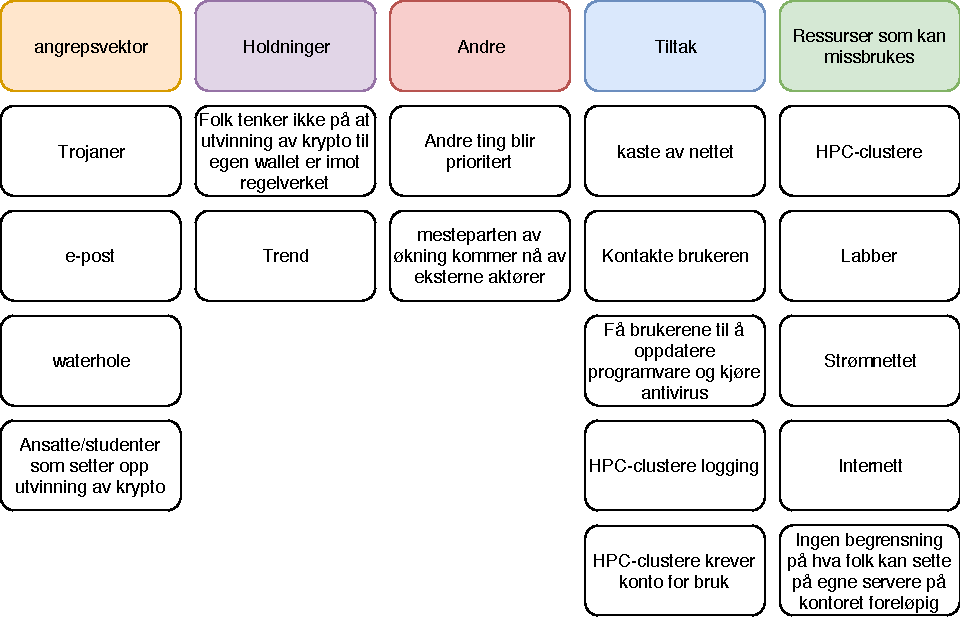
\includegraphics[scale=0.6]{case_3/bilder/AD.pdf}
    \label{fig:AD_miner}
    \caption{Hvordan fungerer utvinning av kryptovaluta ved NTNU?}
\end{figure}

Affinitetsdiagrammet deles inn i hovedkategoriene: angrepsvektor, holdninger, ressurser som kan misbrukes, tiltak og andre. Blant disse er mulige årsaker til problemet og anbefalte tiltak som kan løse det. 



%RESULTAT for affinitetsdiagram.

%%%%%%%%%%%%%%%%%%%%%%%%%%%%%%%%%%%%%%%%%%%%%%%%%%%%%%%%%%%%%%%%%%%%%
\section{Rotårsaksidentifisering}
\subsection{5 whys}
Det ble fremhevet fem årsaker som skulle analyseres. Fire av disse kom fra fiskebeindiagrammet over, og en fra idémyldring. Tabellene under viser resultatene fra gjennomføringen. 

\begin{table} [H]
    \centering
    \begin{tabular}{ | m{5em} | m{30em} | }
        \hline
            \cellcolor{yellow} Årsak: & \cellcolor{yellow} Ansatte og studenter utvinner kryptovaluta med universitetet sine ressurser                \\
        \hline
            Why? & Lønnsomhet                                    \\
        \hline
            Why? & Har ingen utgifter                                            \\
        \hline
            Why? & Bruker strøm og infrastrukturen til universitetet                \\
        \hline
            Why? & Det er en gråsone i regelverket           \\
        \hline
            Why? & Ikke spesifisert godt nok i IT-reglementet   \\
        \hline
    \end{tabular}
    \caption[5 Whys: Ansatte og studenter utvinner kryptovaluta med universitetet]{5 Whys på ansatte og studenter utvinner kryptovaluta med universitetet}
    \label{5Whys-interne}
\end{table}
Det å utvinne kryptovaluta på universitetet sine ressurser er alt fra å kjøre en kryptoutvinner på en PC til å sette opp maskinvare ment for kryptoutvinning. I 5 Whys over kom vi frem til at lønnsomhet er primærgrunnen til at de driver med kryptoutvinning, men årsaken til at ansatte og studenter utvinner på universitet er at det ikke er spesifisert godt nok i IT-reglementet.   


\begin{table} [H]
    \centering
    \begin{tabular}{ | m{5em} | m{30em} | }
        \hline
            \cellcolor{yellow} Årsak: & \cellcolor{yellow} Eksterne trusselaktører utvinner kryptovaluta med universitetet sine ressurser              \\
        \hline
            Why? & Lønnsomhet                                   \\
        \hline
            Why? & Enkelt å spre minere                                           \\
        \hline
            Why? & Folk går inn på waterholes og trykker på phishingmail               \\
        \hline
            Why? & Brukeren var ikke oppmerksom nok på e-post eller siden de gikk på           \\
        \hline
            Why? & Brukere har ikke fått nok opplæring i hvordan dette unngås    \\
        \hline
    \end{tabular}
    \caption[5 Whys: Eksterne trusselaktører utvinner kryptovaluta med universitetet sine ressurser]{5 Whys Eksterne trusselaktører utvinner kryptovaluta med universitetet sine ressurser}
    \label{5Whys-eksterne}
\end{table}

Årsaken til at eksterne trusselaktører utvinner kryptovaluta med universitetet sine ressurser er fordi det er en lønnsom affære som koster lite å distribuere og som det er liten sannsynlighet å bli tatt for. Dette virker i kombinasjon med at brukere ikke er oppmerksom på hva de trykker på. Rotårsaken til at de ikke er oppmerksomme er at de ikke har fått nok opplæring.

\begin{table} [H]
    \centering
    \begin{tabular}{ | m{5em} | m{30em} | }
        \hline
            \cellcolor{yellow} Årsak: & \cellcolor{yellow} Utvinnere som implementert inn i nettsider              \\
        \hline
            Why? & God fortjeneste                                   \\
        \hline
            Why? & Fordi de når en stor menge folk som utvinner kryptovaluta for dem                                           \\
        \hline
            Why? & Mange har ikke en annonseblokkering som også stopper utvinnere på nett               \\
        \hline
            Why? & På grunn av lite eller ingen opplæring til denne typen programvare           \\
        \hline
            Why? & Ikke prioritert    \\
        \hline
            Why? & Fordi det ikke er nok folk/ressurser    \\
        \hline
    \end{tabular}
    \caption[5 Whys: Utvinningsverktøy som er implementert inn i nettsider]{5 Whys på ansatte og studenter utvinner kryptovaluta med universitetet sine ressurser}
    \label{5Whys-minere}
\end{table}

Utvinning på nettsider blir mer utbredt fordi det er profitabelt og en god erstatning til reklame. Dette kan bli stoppet med annonseblokkering eller blokkering av DNS adresser. Dette blir ikke gjort fordi det ikke er en prioritet fra Seksjon for Digital Sikkerhet.

\subsection{Feiltreanalyse}
Feiltreanalyse tar for seg alle mulige årsaker i et diagram og identifiserer mulige relasjoner. Analysen bygger på hva som ble gjort i 5 Whys.

Vi har kommet fram til fire hovedgrunner til at kryptoutvinning på NTNU forekommer. Rotårsaken er sammensatt av årsakene definert i figur \ref{fig:feil_tre_analyse}. I dette caset er problemet delt inn i to deler: de interne og de eksterne. Det er to forskjellige typer årsaker, der interne går mer på regelverk og eksterne er mer teknisk. 

 \begin{figure}[H]
    \centering
    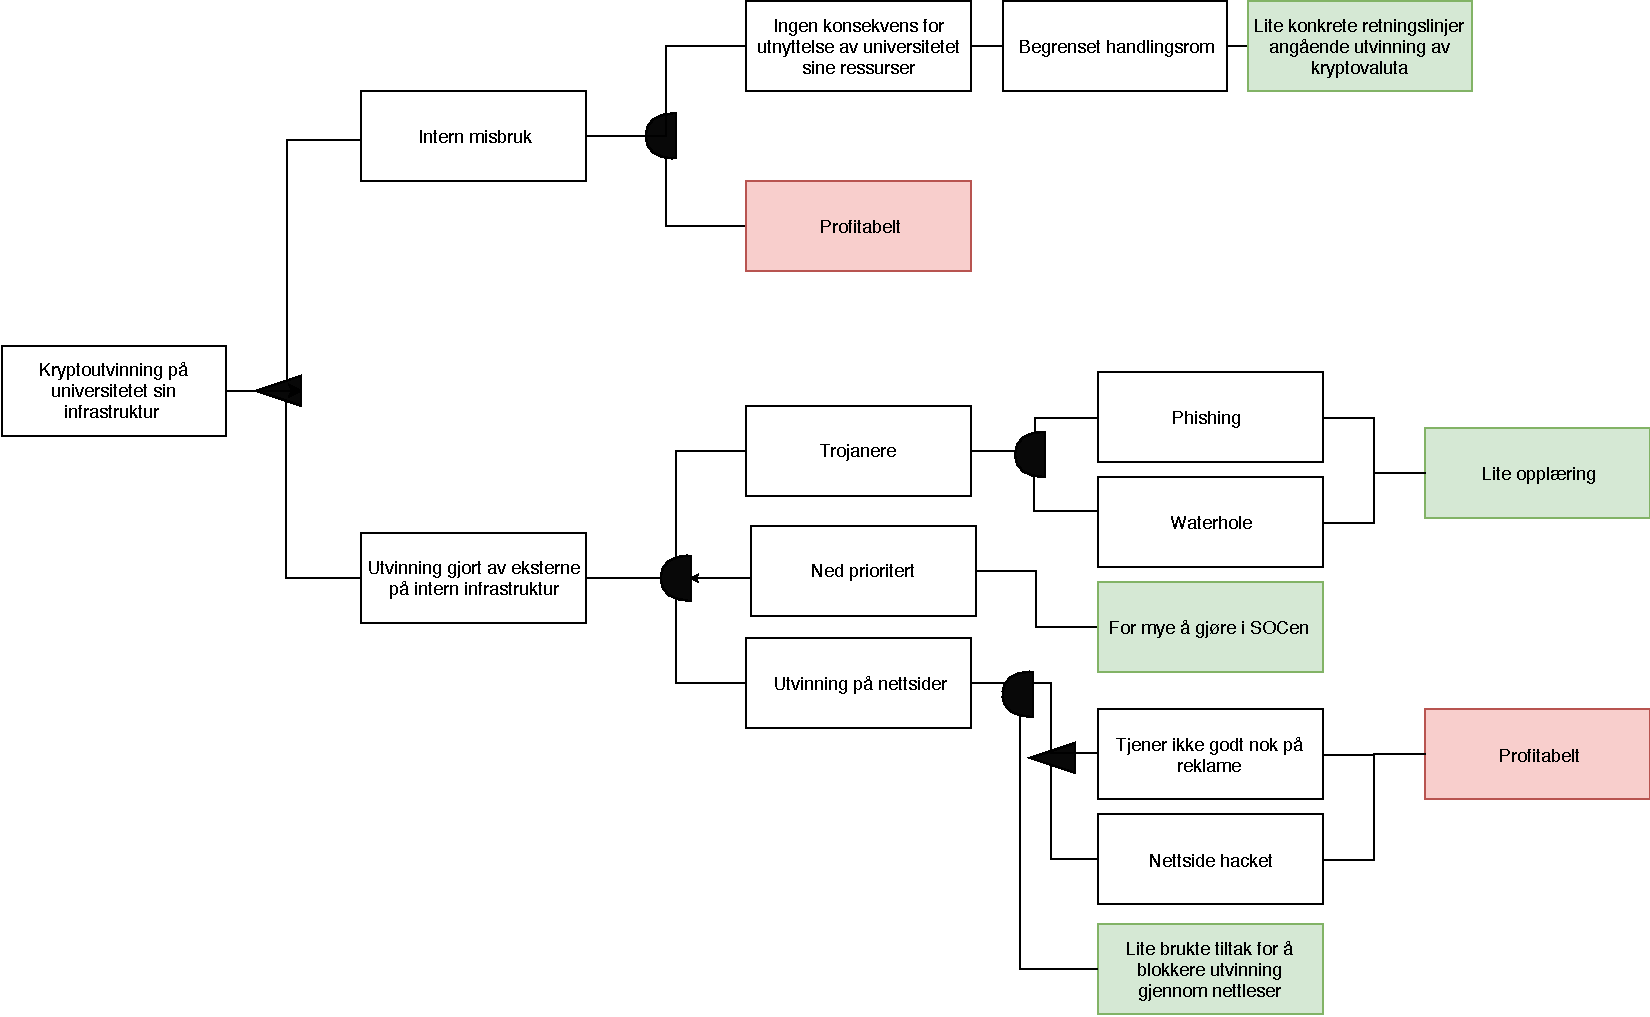
\includegraphics[scale=0.45]{case_3/bilder/feil_tre_analyse.pdf}
    \caption{Feiltreanalyse}
    \label{fig:feil_tre_analyse}
\end{figure}

I figur \ref{fig:feil_tre_analyse} over representerer trekanter ``eller'' og halvsirkelen ``og''. De røde boksene er de årsakene vi ikke kan gjøre noe med, mens de grønne kan det gjøres noe med.
%%%%%%%%%%%%%%%%%%%%%%%%%%%%%%%%%%%%%%%%%%%%%%%%%%%%%%%%%%%%%%%%%%%%%
\section{Rotårsakseliminering}
\subsection{SIT}
Alle komponenter som eksisterer i problemets naturlige omgivelser listes under:

\begin{itemize}
    \item IT-reglement
    \item Annonseblokker
    \item Internett
    \item SOCen
    \item Brannmur
    \item Servere og datamaskiner
    \item Datalabber
    \item HPC-cluster
    \item Bring your own device (BYOD)
    \item Strøm
\end{itemize}

Når komponentene er gjort rede for, vil de fem SIT prinsippene brukes sekvensielt på komponentene for å utvikle løsninger på problemene. Ikke alle SIT-prinsipper finner løsninger som er gjennomførbare for alle komponenter. I disse tilfellene vil det stå: ``Ikke gjennomførbart''. Resultatene fremheves under.

\paragraph{IT-reglement}
\begin{itemize}
    \item \textbf{Attributtavhengighet} Legge til et større fokus på utvinning av kryptovaluta.
    \item \textbf{Komponentkontroll} Gjennomføre en informasjonskampanje for å sette fokus på hva som er misbruk.
    \item \textbf{Erstatning} Ikke gjennomførbart.
    \item \textbf{Forkastning} Ikke gjennomførbart.
    \item \textbf{Oppdeling} Ikke gjennomførbart. 
\end{itemize}

\paragraph{Annonseblokker}
\begin{itemize}
    \item \textbf{Attributtavhengighet} Legge til blokkering av kryptoutvinning 
    \item \textbf{Komponentkontroll} Passe på at alle ansatte har annonseblokker installert som også stopper utvinning av kryptovaluta.
    \item \textbf{Erstatning} Ikke gjennomførtbart
    \item \textbf{Forkastning} Ikke gjennomførtbart
    \item \textbf{Oppdeling} Ikke gjennomførtbart.
\end{itemize}

\paragraph{Internett}
\begin{itemize}
    \item \textbf{Attributtavhengighet} Blokkere kryptoutvinning
    \item \textbf{Komponentkontroll} Automatisere at alle datamaskiner som utvinner kryptovaluta blir kastet av nettet.
    \item \textbf{Erstatning} Ikke gjennomførtbart.
    \item \textbf{Forkastning} Ikke gjennomførtbart.
    \item \textbf{Oppdeling} Ikke gjennomførtbart.
\end{itemize}


\paragraph{SOC}
\begin{itemize}
    \item \textbf{Attributtavhengighet} Øke antall ansatte.
    \item \textbf{Komponentkontroll} Økt prioritet til kryptovaluta.
    \item \textbf{Erstatning} Ikke gjennomførtbart.
    \item \textbf{Forkastning} Ikke gjennomførtbart.
    \item \textbf{Oppdeling} Gi forslag til implementering av tiltak til bachelorgrupper.
\end{itemize}

\paragraph{Servere og datamaskin}
\begin{itemize}
    \item \textbf{Attributtavhengighet} Strengere adgangskontroll.
    \item \textbf{Komponentkontroll} Ikke gjennomførtbart.
    \item \textbf{Erstatning} Ikke gjennomførtbart.
    \item \textbf{Forkastning} Ikke gjennomførtbart.
    \item \textbf{Oppdeling} Ikke gjennomførtbart.
\end{itemize}

\paragraph{Datalabber}
\begin{itemize}
    \item \textbf{Attributtavhengighet} Strengere adgangskontroll.
    \item \textbf{Komponentkontroll} Logging.
    \item \textbf{Erstatning} Svakere maskinvare på labbene.
    \item \textbf{Forkastning} Slutte å tilby labber, som kan brukes i sammenheng med kryptoutvinning.
    \item \textbf{Oppdeling} Ikke gjennomførbart.
\end{itemize}

\paragraph{HPC-clustere}
\begin{itemize}
    \item \textbf{Attributtavhengighet} Øke tilgangskontrollen ytterligere.
    \item \textbf{Komponentkontroll} Ikke gjennomførbart.
    \item \textbf{Erstatning} Ikke gjennomførbart.
    \item \textbf{Forkastning} Ikke gjennomførbart.
    \item \textbf{Oppdeling} Ikke gjennomførbart.
\end{itemize}


\paragraph{Bring your own device (BYOD)}
\begin{itemize}
    \item \textbf{Attributtavhengighet} Ikke gjennomførbart.
    \item \textbf{Komponentkontroll} Kaste datamaskiner som ikke tilhører NTNU-personell av nettet slik at de manuelt må koble seg på igjen.
    \item \textbf{Erstatning} Ikke gjennomførbart.
    \item \textbf{Forkastning} Ikke gjennomførbart.
    \item \textbf{Oppdeling} Ikke gjennomførbart.
\end{itemize}

\paragraph{Strøm}
\begin{itemize}
    \item \textbf{Attributtavhengighet} Ikke gjennomførtbart
    \item \textbf{Komponentkontroll} Strømkvotering, overstiges kvoten må vedkommende betale for strømmen
    \item \textbf{Erstatning} Ikke gjennomførtbart
    \item \textbf{Forkastning} Ikke gjennomførtbart
    \item \textbf{Oppdeling} Ikke gjennomførtbart
\end{itemize}

Vi sorterer og beskriver de mest relevante idéer til videre utdyping:

\begin{description}
\item[Gjennomføre en informasjonskampanje om kommersielt misbruk av NTNU sin infrastruktur] Kampanjen skal få frem at det å bruke NTNU sine ressurser til kommersiell virksomhet bryter IT-reglementet. I NTNU sine ressurser inkluderer strøm og internett. %(y)
\item[Legge til et større fokus på utvinning av kryptovaluta i IT-reglementet] Gi IT-reglement et større fokus på kryptoutvinning og gi klarere retningslinjer på hva som ikke er akseptabelt.
\item[Legge til annonseblokker som stopper utvinning] Aktivere blokkering av utvinningsprotokoll på annonseblokkere og passe på at alle har en annonseblokkeringstjeneste installert.
\item[Blokkere kryptoutvinning] Med dette mener vi å gjøre et eller flere tiltak som å blokkere DNS-forespørsler som omhandler kryptoutvinning.  
\item[Øke antall personell i SOC] SOC har mange oppgaver som er mer kritiske enn kryptoutvinning. Derfor foreslår vi å ansette flere, kanskje i kombinasjon med bacheloroppgaver.
\item[Strengere adgangskontroll] Begrenser tilgang til datalabber. 
\item[Logging] Øke bruk av logging i datalabbene. 
\item[Kaste datamaskiner som ikke er kritisk infrastruktur av nettet] Ved midnatt blir alle datamaskiner eller servere som ikke er kritisk infrastruktur koblet av nettet og må manuelt koble seg på nettet igjen.
\end{description}

\subsection{Tiltaksplan}
Etter å ha brukt de fem SIT-prinsippene på hver komponent og filtrert de, sitter vi igjen med et par idéer. I denne delen fremhever vi idéer i en tiltaksplan som vi anbefaler å implementere. 
Under beskrives de ulike tiltakene:

\begin{description}
    \item[Gjennomføre en informasjonskampanje om kommersielt misbruk av NTNU sin infrastruktur] Utvinning av kryptovaluta er en ny ting, hvor mange ikke er klar over hvordan universitetet sitt regelverk håndterer temaet. Vår anbefaling er å ha en kampanje der universitet informerer om hva som regnes som NTNU sine ressuser og hvordan disse ikke skal brukes til kommersiell virksomhet.
    \item[Legge til et større fokus på utvinning av kryptovaluta i IT-reglementet] Endre IT-reglementet slik at det blir tydelig at kryptoutvinning ikke er lovlig bruk av NTNU sine ressurser. 
    \item[Blokkere kryptoutvinning] Dette tiltaket går ut på å blokkere DNS-forespørsler tilknyttet kryptoutvinning. Slik at PCer som blir brukt i utvinning ikke kan hente nye oppgaver å løse. De velkjente DNS-ene blokkeres. Videre kan loggen bli benyttet for å legge nye domener inn i en svarteliste, eller justere de gamle DNS-ene.
    \item[Øke antall personell i SOC] SOCen kan ikke prioritere å stoppe utvinning av kryptovaluta. Derfor anbefaler vi å enten øke mengden personell i SOCen, eller gi utvikling av et teknisk forslag til implementasjon som en bacheloroppgave.
\end{description}

%%%%%%%%%%%%%%%%%%%%%%%%%%%%%%%%%%%%%%%%%%%%%%%%%%%%%%%%%%%%%%%%%%%%%
\section{Løsningsimplementering}
\subsection{Kraftfeltsanalyse} 
Kraftfeltsanalyse blir brukt for å få en oversikt over hvilke styrker som er for og hvilke styrker som er mot implementering av tiltakene. Dette verktøyet gir en plan over hvilke tiltak som er lettest å gjennomføre.  

Informasjonskampanjen og endringen i IT-reglementet bør gjøre i kombinasjon med hverandre. Der IT-reglementet får klartgjort at selv om kryptoutvinning ikke ulovlig i henhold til norsk lov, er det imot NTNU sitt IT-reglement så fremt det ikke er søkt om. Når endringen er gjort, gjennomføres informasjonskampanjen.   
Under, i tabell \ref{fig:kampanje} og \ref{fig:IT-reglement}, viser resultatene fra kraftfeltsanalysen på informasjonskampanje og endring i IT-reglementet.
 \begin{figure}[H]
    \hspace{2.2cm}
    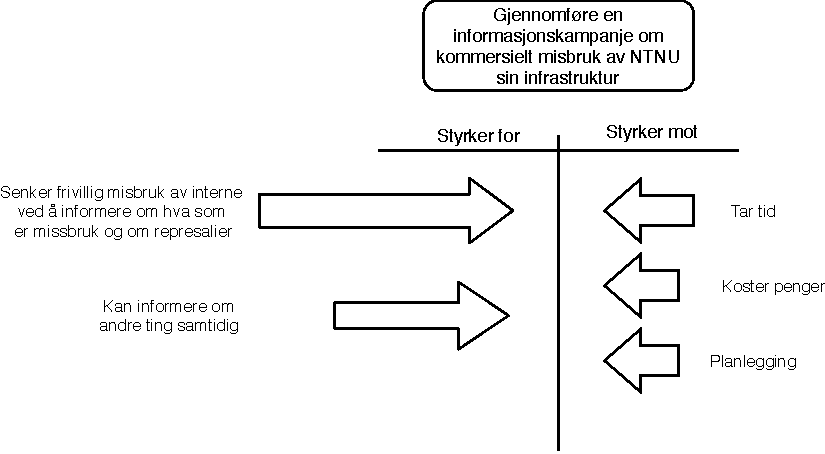
\includegraphics[scale=0.6]{case_3/bilder/Force-field1.pdf}
    \caption[Informasjonskampanje]{Oversikt over informasjonskampanjen }
    \label{fig:kampanje}
\end{figure}

 
 \begin{figure}[H]
    \hspace{2.6cm}
    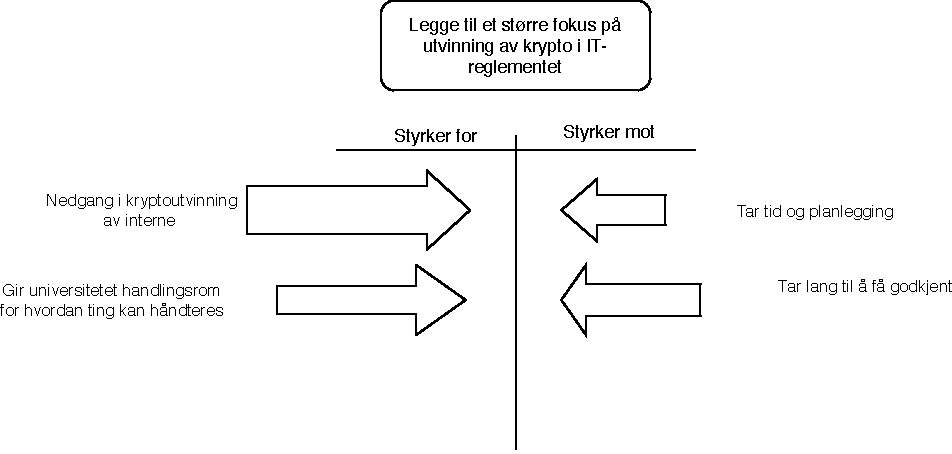
\includegraphics[scale=0.6]{case_3/bilder/Force-field2.pdf}
    \caption[Endre IT-reglementet]{Endring i IT-reglementet}
    \label{fig:IT-reglement}
\end{figure}

Fra dataanalysen kom vi frem til at selv om det finnes tekniske løsninger, har ikke SOCen hatt mulighet til å implementere DNS blokkering på bakgrunn av mangel på ressurser. Figur \ref{fig:Blokkering} og \ref{fig:Oke-antall} viser hva som skal til for å blokkere DNS og hva som må til for å øke ressursene til SOCen. Vi estimerer at den største kraften mot implementering av dette kommer til å være tidsbruk og kostnadene rundt tidsbruk.    
 \begin{figure}[H]
    \centering
    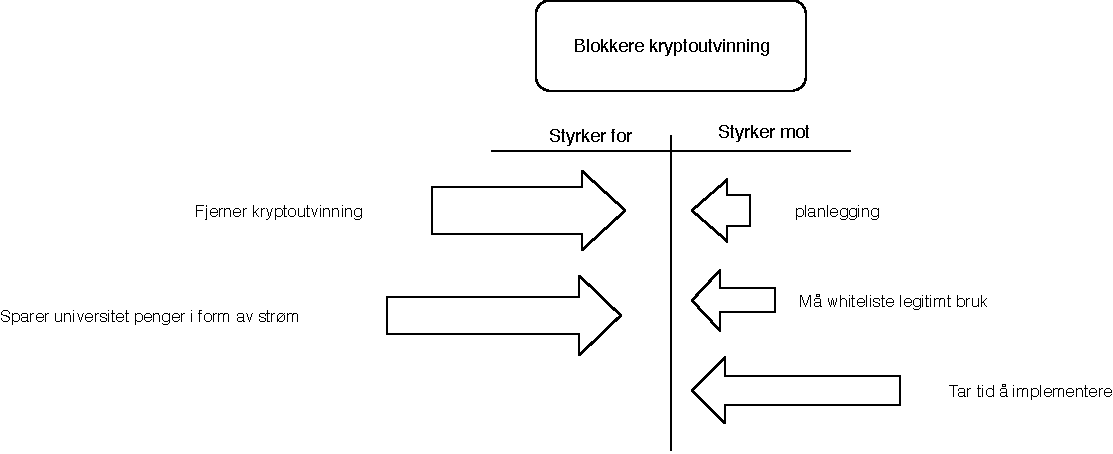
\includegraphics[scale=0.6]{case_3/bilder/Force-Field3.pdf}
    \caption[Blokkering]{Blokkering av DNS forespørsel}
    \label{fig:Blokkering}
\end{figure}


Ved å øke antall ansatte i SOCen estimerer vi at kosten av en ny ansatt vil være største kraften mot. Det er vanskelig å si om vedkommende vil ha nok arbeidsoppgaver til at det er verdt ansettelsen. Det bør vurderes å gi prosjekter til bachelor- og masterstudenter. 
 \begin{figure}[H]
    \hspace{3.6cm}
    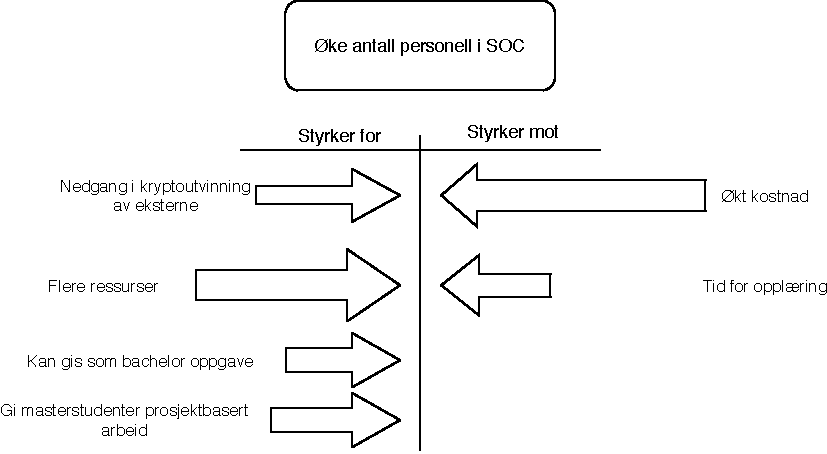
\includegraphics[scale=0.6]{case_3/bilder/Force-field4.pdf}
    \caption[Øke antall ansette i SOC]{Øke andel ansatte i SOC}
    \label{fig:Oke-antall}
\end{figure}

Figurene viser våres antakelser på hvilke krefter som jobber for implementeringen og hvilke som jobber mot, samt estimater på styrken til kreftene. Lengden på pilene indikerer antatt styrke. 
%%%%%%%%%%%%%%%%%%%%%%%%%%%%%%%%%%%%%%%%%%%%%%%%%%%%%%%%%%%%%%%%%%%%%
\section{Kostnad-nytte-analyse}
\label{kost-nytte-case3}
Denne seksjonen tar for seg en kostnad-nytte-analyse av nytteverdien til bruk av rotårsaksanalyse for case 3. 

\subsection{Kostnad for gjennomføring}
I denne analysen definerer vi kostnad som tid brukt på en iterasjonen av metoden. Vi definerer en skala for kostnad fra 1 til 5 der nivåene tilsvarer følgende tidsbruk:

\begin{enumerate}
    \item Under 50 timer
    \item 50-150 timer
    \item 150-250 timer
    \item 250-400 timer
    \item Over 400 timer
\end{enumerate}

Tabell \ref{tab:tidsbruk_case3} under viser tidsbruken i enkeltfasene i dette caset. Dette inkluderer tid brukt til å dokumentere alt som har med de enkelte fasene å gjøre. 

% Table generated by Excel2LaTeX from sheet 'Ark1'
\begin{table}[H]
  \centering
  \caption{Tidsbruk i de ulike fasene i case 3}
    \begin{tabular}{|lr|l|}
    \hline
    \multicolumn{3}{|c|}{\cellcolor{yellow}\textbf{Case 3}} \\
    \hline
    \multicolumn{1}{|l|}{\cellcolor{apricot}\textbf{Fase}} & \multicolumn{1}{l|}{\cellcolor{apricot}\textbf{Verktøy brukt}} & \cellcolor{apricot}\textbf{Timer totalt} \\
    \hline
    \multicolumn{1}{|l|}{Problemforståelse} & \multicolumn{1}{l|}{Ytelsesmatrise} & 16-20t \\
    \hline
    \multicolumn{1}{|l|}{Idémyldring} & \multicolumn{1}{l|}{Idémyldring og NGT} & 16-20t \\
    \hline
    \multicolumn{1}{|l|}{Datainnsamling} & \multicolumn{1}{l|}{Intervju} & 20-30t \\
    \hline
    \multicolumn{1}{|l|}{Datanalyse} & \multicolumn{1}{l|}{Affinitetsdiagram} & 15-20t \\
    \hline
    \multicolumn{1}{|l|}{Rotårsaksidentifisering} & \multicolumn{1}{l|}{5 whys og feil-tre diagram} & 25-30t \\
    \hline
    \multicolumn{1}{|l|}{Rotårsakseliminering} & \multicolumn{1}{l|}{SIT} & 15-20t \\
    \hline
    \multicolumn{1}{|l|}{Løsningsimplementering} & \multicolumn{1}{l|}{Kraftfeltsdiagram} & 10-15t \\
    \hline
    \multicolumn{2}{|l|}{\textbf{Sum}} & \textbf{117-155t} \\
    \hline
    \end{tabular}%
  \label{tab:tidsbruk_case3}%
\end{table}%

Dersom kosten på caset går over flere nivåer regner vi med medianen til ytterpunktene for å plassere kostnaden. Basert på kostnadsnivåene vi definerte over, plasseres tidsbruken på case 3 til:
\[Kostnad = 2\]

\subsection{Nytte av resultatene}
I denne analysen definerer vi nytten som egen oppfatning av hvor gode resultatene fra caset var. Det vurderes ut fra om vi tror det kan finnes andre underliggende årsaker, og hvorvidt vi mener problemet blir løst dersom rotårsakene fjernes. Nytten defineres på en skala fra 1 til 5. 

I dette caset kom vi frem til at rotårsakene var uklarhetet i IT-reglement når det kommer til utvinning av kryptovaluta, samt for lite ressurser på Seksjon for Digital Sikkerhet for å gjøre noe med tekniske løsninger. Caset ble preget av svakt datagrunnlag, så vi har grunn til å tro at det kan være flere rotårsaker. Tiltakene vi kom frem til vil kunne hjelpe med å begrense konsekvensene til problemet, men vil trolig ikke fjerne det helt. Vi definerer derfor nytten til:
\[Nytte = 2\]

\subsection{Total nytteverdi}
Når vi regner ut kostnad-nytte deler vi kostnaden på nytteverdien. 
\[\frac{Kostnad}{Nytte} = Total nytteverdi\]

I dette caset blir regnestykket slik:
\[\frac{2}{2} = 1\]

Svarene på regnestykket kan bli fra 0,2 til 5. Jo lavere denne nytteverdien er, jo bedre fungerte metoden til caset. 